\documentclass{beamer}
\usepackage[T1]{fontenc}
\usepackage{hyperref}
\usepackage{tkz-graph}
\usepackage[linesnumbered,ruled, longend]{algorithm2e}
\usepackage{gensymb}

\usetheme{Warsaw}
\usecolortheme{}
\useoutertheme{infolines}
%%\setbeamertemplate{footline}[title in head,frame number]
\title{- Soutenance de projet -  }
\setbeamertemplate{footline}
{
  \leavevmode%
  \hbox{%
  \begin{beamercolorbox}[wd=.5\paperwidth,ht=2.25ex,dp=1ex,center]{title in head/foot}%
    \usebeamerfont{title in head/foot}\insertshortsubtitle
  \end{beamercolorbox}%
  \begin{beamercolorbox}[wd=.5\paperwidth,ht=2.25ex,dp=1ex,right]{date in head/foot}%
    \usebeamerfont{date in head/foot}\insertshortdate{}\hspace*{2em}
    \insertframenumber{} / \inserttotalframenumber\hspace*{2ex} 
  \end{beamercolorbox}}%
  \vskip0pt%
}
\setbeamertemplate{navigation symbols}{}
\subtitle{Solveur de Ricochet Robots}
\author{Erwan Philippe MENSAH  \\ TOURE Papa Samba Khary \\ TRAORE Daouda}
\institute{L2 Informatique \\ Groupe 2A}
\date{}


\begin{document}
%---------------------------------------------------------------
\begin{frame}
	\begin{figure}
        
\includegraphics[scale=0.14]{Images/logo.jpg}
	\end{figure}
	\titlepage
\end{frame}

%---------------------------------------------------------------
\section{Sommaire}
    \begin{frame}{Sommaire}
        \tableofcontents
    \end{frame}
%---------------------------------------------------------------
\section{Introduction}
    \begin{frame}{Introduction}
        \begin{itemize}
            \item Le Ricochet Robots: jeu de société composé d'un plateau, de quatre de robots et de 17 jetons. 
            \vspace{0.25cm}
            \item Principe: Déplacer les robots pour atteindre la case qui correspond au symbole du jeton ayant été tiré aléatoirement.
             Le déplacement des robots s'effectue qu'en ligne droite jusqu'à rencontrer un obstacle (un robot ou un mur).
            
            \vspace{0.25cm}
            
            \item Objectifs: 
            \begin{itemize}
                \item Conception du Ricochet Robots.
                \item Réalisation d'une interface graphique.
                \item Implémentation de l'algorithme A*, optimisation de l'algorithme.
            \end{itemize}
        \end{itemize}
    \end{frame}
%---------------------------------------------------------------
    \begin{frame}{Exemple de Plateau}
        \begin{figure}
            \centering
            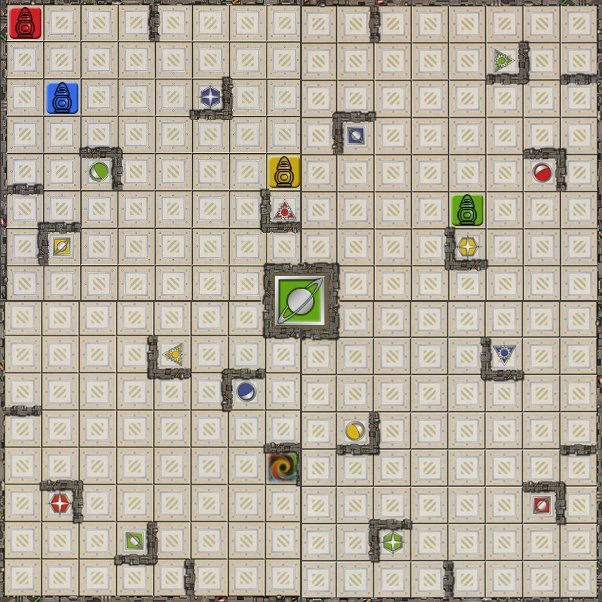
\includegraphics[scale=0.2]{Images/palteau3.jpg}
        \end{figure}
        \begin{block}{Remarque}
            Nous avons 96 configurations possibles.
        \end{block}
    \end{frame}
%---------------------------------------------------------------
\section{Principe du jeu}
\begin{frame}{Principe du jeu}
    \begin{columns}
        \begin{column}{0.6\textwidth}
        \vspace{\topsep}
        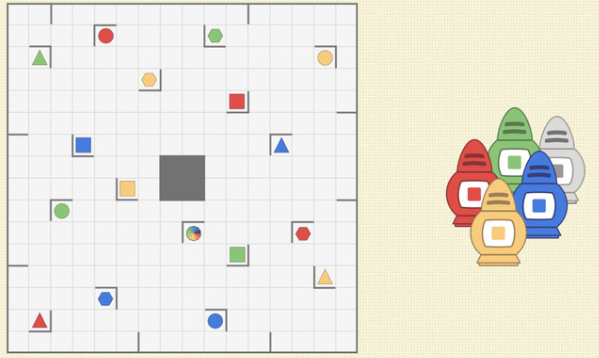
\includegraphics[width=\columnwidth]{Images/r1.png}%
        \end{column}
        
        \begin{column}{0.4\textwidth}
        \begin{itemize}
        \item Comment cela fonctionne?
        \end{itemize}
        \end{column}
    \end{columns}
\end{frame}
%---------------------------------------------------------------
\begin{frame}{Principe du jeu}
    \begin{columns}
        \begin{column}{0.6\textwidth}
        \vspace{\topsep}
        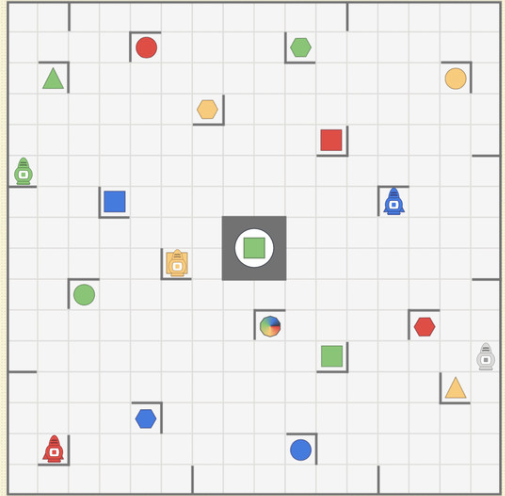
\includegraphics[scale=0.4]{Images/r2.png}%
        \end{column}
        
        \begin{column}{0.4\textwidth}
        \begin{itemize}
        \item Mouvements pour amener le robot \textcolor{green}{Vert} à la cible \textcolor{green}{carré verte}.
        \end{itemize}
        \end{column}
    \end{columns}
\end{frame}
%---------------------------------------------------------------
\begin{frame}{Principe du jeu}
    \begin{columns}
        \begin{column}{0.6\textwidth}
        \vspace{\topsep}
        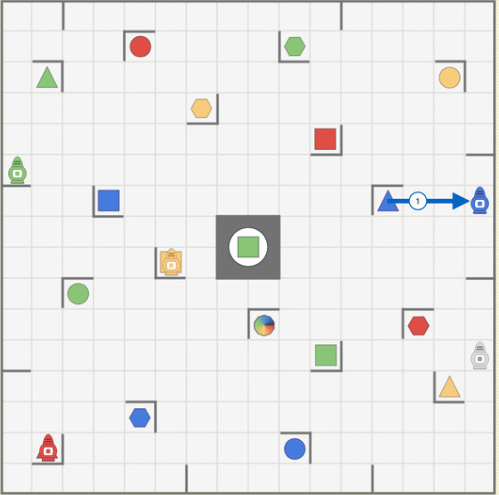
\includegraphics[scale=0.4]{Images/r3.png}%
        \end{column}
        
        \begin{column}{0.4\textwidth}
        \begin{itemize}
        \item Mouvements pour amener le robot \textcolor{green}{Vert} à la cible \textcolor{green}{carré verte}
        \item \textcolor{blue}{Bleu} $\longleftrightarrow$ \textcolor{blue}{droite}
        \end{itemize}
        \end{column}
    \end{columns}
\end{frame}
%---------------------------------------------------------------
\begin{frame}{Principe du jeu}
    \begin{columns}
        \begin{column}{0.6\textwidth}
        \vspace{\topsep}
        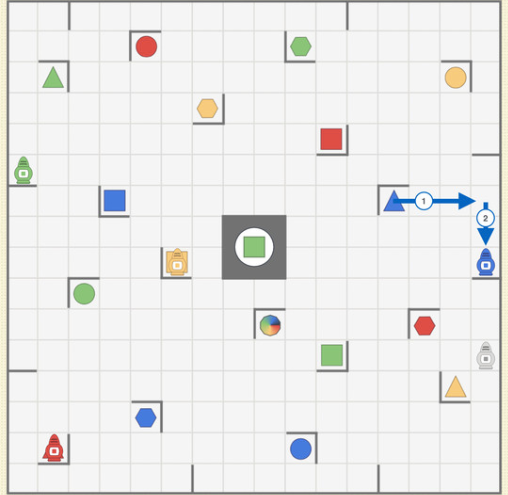
\includegraphics[scale=0.4]{Images/r4.png}%
        \end{column}
        
        \begin{column}{0.4\textwidth}
        \begin{itemize}
        \item Mouvements pour amener le robot \textcolor{green}{Vert} à la cible \textcolor{green}{carré verte}.
        \item \textcolor{blue}{Bleu} $\longleftrightarrow$ \textcolor{blue}{droite}
        \item \textcolor{blue}{Bleu} $\longleftrightarrow$ \textcolor{blue}{bas}
        \end{itemize}
        \end{column}
    \end{columns}
\end{frame}
%---------------------------------------------------------------
\begin{frame}{Principe du jeu}
    \begin{columns}
        \begin{column}{0.6\textwidth}
        \vspace{\topsep}
        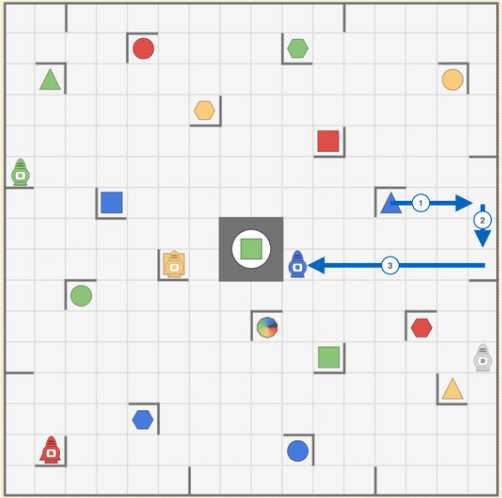
\includegraphics[scale=0.4]{Images/r5.png}%
        \end{column}
        
        \begin{column}{0.4\textwidth}
        \begin{itemize}
        \item Mouvements pour amener le robot \textcolor{green}{Vert} à la cible \textcolor{green}{carré verte}.
        \item \textcolor{blue}{Bleu} $\longleftrightarrow$ \textcolor{blue}{droite}
        \item \textcolor{blue}{Bleu} $\longleftrightarrow$ \textcolor{blue}{bas}
        \item \textcolor{blue}{Bleu} $\longleftrightarrow$ \textcolor{blue}{gauche}
        \end{itemize}
        \end{column}
    \end{columns}
\end{frame}
%---------------------------------------------------------------
\begin{frame}{Principe du jeu}
    \begin{columns}
        \begin{column}{0.6\textwidth}
        \vspace{\topsep}
        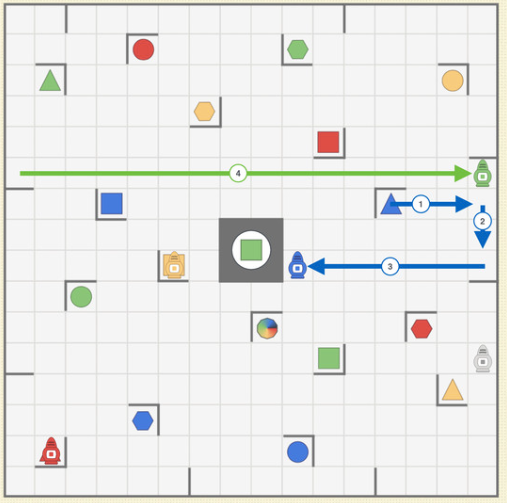
\includegraphics[scale=0.4]{Images/r6.png}%
        \end{column}
        
        \begin{column}{0.4\textwidth}
        \begin{itemize}
        \item Mouvements pour amener le robot \textcolor{green}{Vert} à la cible \textcolor{green}{carré verte}.
        \item \textcolor{blue}{Bleu} $\longleftrightarrow$ \textcolor{blue}{droite}
        \item \textcolor{blue}{Bleu} $\longleftrightarrow$ \textcolor{blue}{bas}
        \item \textcolor{blue}{Bleu} $\longleftrightarrow$ \textcolor{blue}{gauche}
        \item \textcolor{green}{Vert} $\longleftrightarrow$ \textcolor{green}{droite}
        \end{itemize}
        \end{column}
    \end{columns}
\end{frame}
%---------------------------------------------------------------
\begin{frame}{Principe du jeu}
    \begin{columns}
        \begin{column}{0.6\textwidth}
        \vspace{\topsep}
        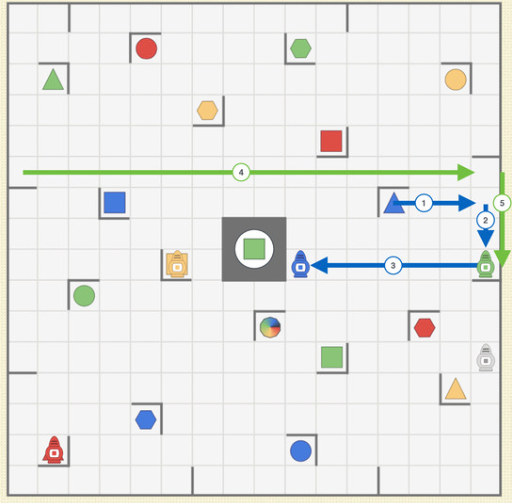
\includegraphics[scale=0.4]{Images/r7.png}%
        \end{column}
        
        \begin{column}{0.4\textwidth}
        \begin{itemize}
        \item Mouvements pour amener le robot \textcolor{green}{Vert} à la cible \textcolor{green}{carré verte}.
        \item \textcolor{blue}{Bleu} $\longleftrightarrow$ \textcolor{blue}{droite}
        \item \textcolor{blue}{Bleu} $\longleftrightarrow$ \textcolor{blue}{bas}
        \item \textcolor{blue}{Bleu} $\longleftrightarrow$ \textcolor{blue}{gauche}
        \item \textcolor{green}{Vert} $\longleftrightarrow$ \textcolor{green}{droite}
        \item \textcolor{green}{Vert} $\longleftrightarrow$ \textcolor{green}{bas}
        \end{itemize}
        \end{column}
    \end{columns}
\end{frame}
%---------------------------------------------------------------
\begin{frame}{Principe du jeu}
    \begin{columns}
        \begin{column}{0.6\textwidth}
        \vspace{\topsep}
        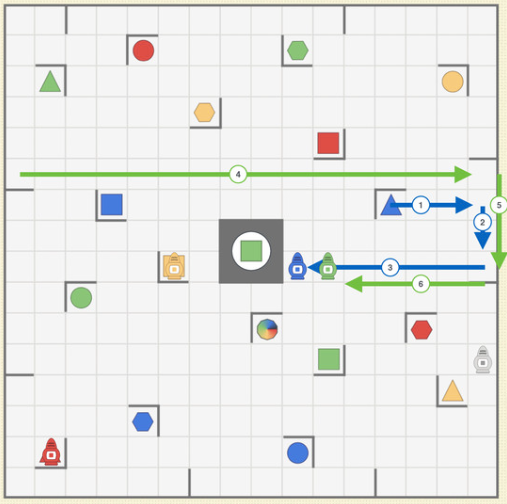
\includegraphics[scale=0.4]{Images/r8.png}%
        \end{column}
        
        \begin{column}{0.4\textwidth}
        \begin{itemize}
        \item Mouvements pour amener le robot \textcolor{green}{Vert} à la cible \textcolor{green}{carré verte}.
        \\item \textcolor{blue}{Bleu} $\longleftrightarrow$ \textcolor{blue}{droite}
        \item \textcolor{blue}{Bleu} $\longleftrightarrow$ \textcolor{blue}{bas}
        \item \textcolor{blue}{Bleu} $\longleftrightarrow$ \textcolor{blue}{gauche}
        \item \textcolor{green}{Vert} $\longleftrightarrow$ \textcolor{green}{droite}
        \item \textcolor{green}{Vert} $\longleftrightarrow$ \textcolor{green}{bas}
        \item \textcolor{green}{Vert} $\longleftrightarrow$ \textcolor{green}{gauche}
        \end{itemize}
        \end{column}
    \end{columns}
\end{frame}
%---------------------------------------------------------------
\begin{frame}{Principe du jeu}
    \begin{columns}
        \begin{column}{0.6\textwidth}
        \vspace{\topsep}
        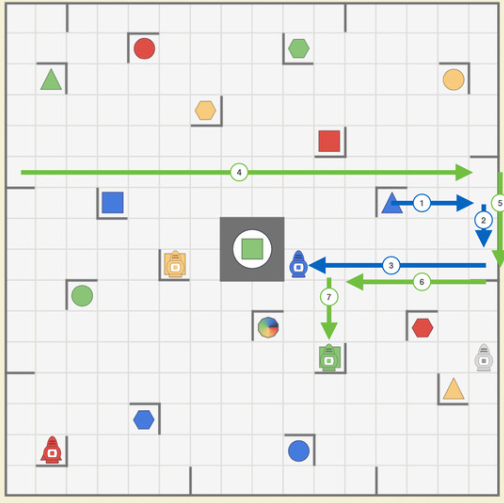
\includegraphics[scale=0.4]{Images/r9.png}%
        \end{column}
        
        \begin{column}{0.4\textwidth}
        \begin{itemize}
        \item Mouvements pour amener le robot \textcolor{green}{Vert} à la cible \textcolor{green}{carré verte}.
        \item \textcolor{blue}{Bleu} $\longleftrightarrow$ \textcolor{blue}{droite}
        \item \textcolor{blue}{Bleu} $\longleftrightarrow$ \textcolor{blue}{bas}
        \item \textcolor{blue}{Bleu} $\longleftrightarrow$ \textcolor{blue}{gauche}
        \item \textcolor{green}{Vert} $\longleftrightarrow$ \textcolor{green}{droite}
        \item \textcolor{green}{Vert} $\longleftrightarrow$ \textcolor{green}{bas}
        \item \textcolor{green}{Vert} $\longleftrightarrow$ \textcolor{green}{gauche}
        \item \textcolor{green}{Vert} $\longleftrightarrow$ \textcolor{green}{bas}
        \end{itemize}
        \end{column}
    \end{columns}
\end{frame}

%---------------------------------------------------------------
\section{Organisation}
\subsection{packages}
\begin{frame}{Les packages}
    \begin{block}{Six packages}
        \begin{itemize}
            \item \textbf{\textit{Game}} : le moteur du jeu
            \item \textbf{\textit{tab}} : création du plateau
            \item \textbf{\textit{view}} : partie graphique
            \item \textbf{\textit{algo}} : AStar
            \item \textbf{\textit{util}} : implémentation MVC
            \item \textbf{\textit{main}} : qui contient l'exécutable de l'application.
        \end{itemize}
    \end{block}
    
\end{frame}
%---------------------------------------------------------------
\begin{frame}{UML du projet}
    \begin{figure}
        \centering
        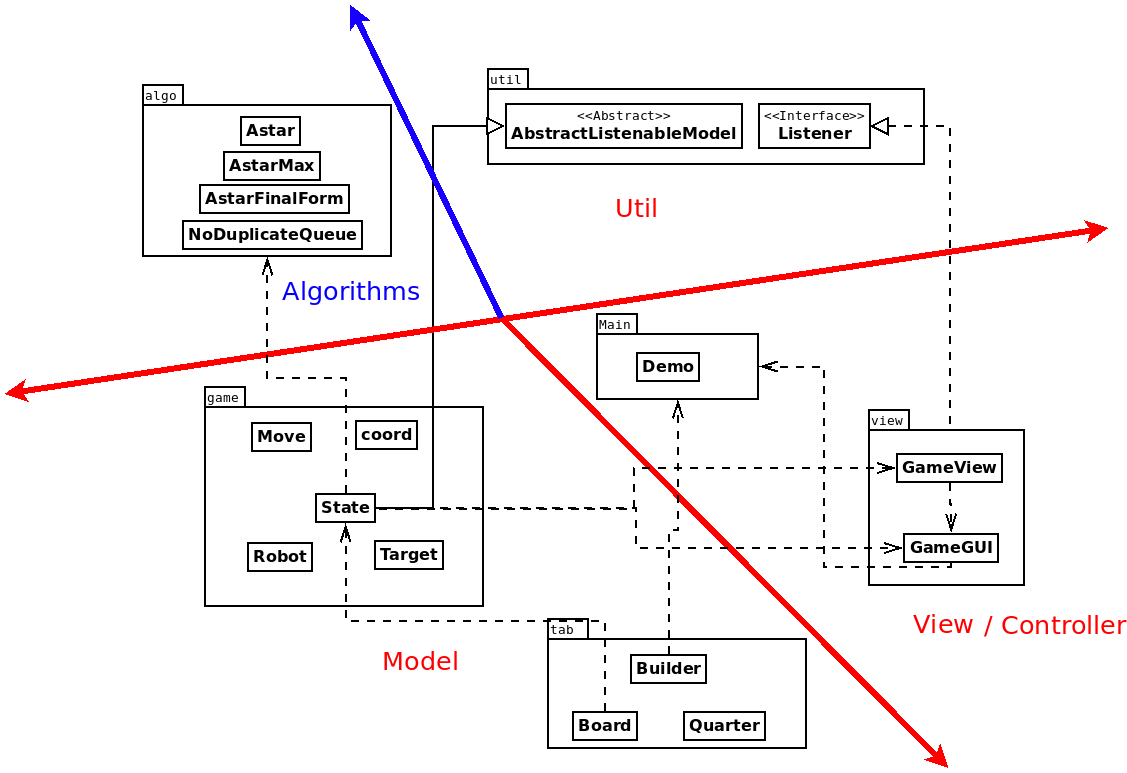
\includegraphics[scale=0.26]{Images/package.png}
    \end{figure}
\end{frame}

%-----------------------------------------------------------------
\section{Réalisation du moteur}
    \subsection{Réalisation du plateau}
        \subsubsection{Représentation d'un case}
            \begin{frame}{Représentation d'un case}
                \begin{itemize}
                    \item \textbf{'N'} indique la présence d'un mur au nord de la case.
                    \item \textbf{'S'} indique la présence d'un mur au sud de la case.
                    \item \textbf{'E'} indique la présence d'un mur à l'est de la case.
                    \item \textbf{'W'} indique la présence d'un mur à l'ouest de la case.
                    \item \textbf{'X'} indique que la case vide.
                    \item les lettres \textbf{'R', 'B', 'G', 'Y'} désignent respectivement les couleurs des targets \textbf{red, blue, yellow, green}
                    \item les lettres \textbf{'C', 'T', 'H', 'Q'} désignent respectivement la forme des targets \textbf{circle, triangle, hexagone, square} 
                \end{itemize}	
            \end{frame}
%---------------------------------------------------------------
            \begin{frame}{Exemple de case}
                    \begin{tikzpicture}
                        \draw (1,1) rectangle (5,5);
                        \draw[color=red] (1,1.5) -- (5,1.5);
                        \draw[color=green] (1,4.5) -- (5,4.5);
                        \draw[color=blue] (1.5,1) -- (1.5,5);
                        \draw[color=olive] (4.5,5) -- (4.5,1);
                        \node[color=red] (pos) at (3,0.5) {SUD};
                        \node[color=green] (pos) at (3,5.5) {NORD};
                        \node[color=blue] (pos) at (0,3) {OUEST};
                        \node[color=olive] (pos) at (6,3) {EST};
                        
                        \node (posi) at (10,5) {["\textbf{NESW}" ]};
                        \draw[->] (5,4) -- (posi);
                    \end{tikzpicture}
                
                \begin{figure}[H]
                    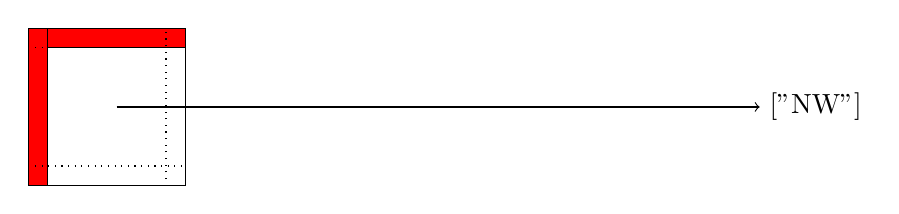
\begin{tikzpicture} 
                        \draw[fill=red] (0,2) rectangle (2, 1.75);
                        \draw[fill=red] (0,0) rectangle (0.25, 2);
    
                        \draw (0,0) rectangle (2,2);
                        \draw[dotted] (0,0.25) -- (2,0.25);
                        \draw[dotted] (0,1.75) -- (2,1.75);
                        \draw[dotted] (0.25,0) -- (0.25,2);
                        \draw[dotted] (1.75,0) -- (1.75,2);
                        
                        \node (void) at (1,1) {};
                        \node (str) at (10,1) {["NW"]};
                        \draw[->] (void) -- (str);
                    \end{tikzpicture}
                \end{figure}
            \end{frame}
%---------------------------------------------------------------            
        \subsubsection{Assemblage des quartiers}
        \begin{frame}{Quartiers}
            \begin{block}{Composition}
                Le plateau est composé de 4 quartiers pouvant être placés aléatoirement.
            \end{block}
            \begin{center}
                \begin{tikzpicture}
                    \draw (0,0) rectangle (4,4);
                    \draw[dotted] (0,2) -- (4,2);
                    \draw[dotted] (2,0) -- (2,4);
                    \node (4) at (1,1) {4};
                    \node (3) at (3,1) {3};
                    \node (2) at (3,3) {2};
                    \node (1) at (1,3) {1};
                \end{tikzpicture}
            \end{center}
        \end{frame}
%---------------------------------------------------------------        
        \begin{frame}{Placement et rotation des quartiers}
            \begin{itemize}
                \item Premier quartier inchangé.
                \item Second : rotation de 90\degree
                \item Troisième : double rotation de 90\degree
                \item Quatrième : triple rotation de 90\degree
            \end{itemize}
            \begin{figure}
                \centering
                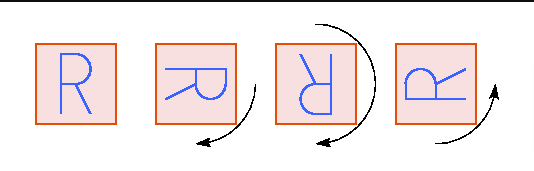
\includegraphics[scale=0.5]{Images/rota.png}
            \end{figure}
        \end{frame}
 
%---------------------------------------------------------------        
    \subsection{Mouvements Robots}    
        \begin{frame}{Déplacement Robots}
            \centering
            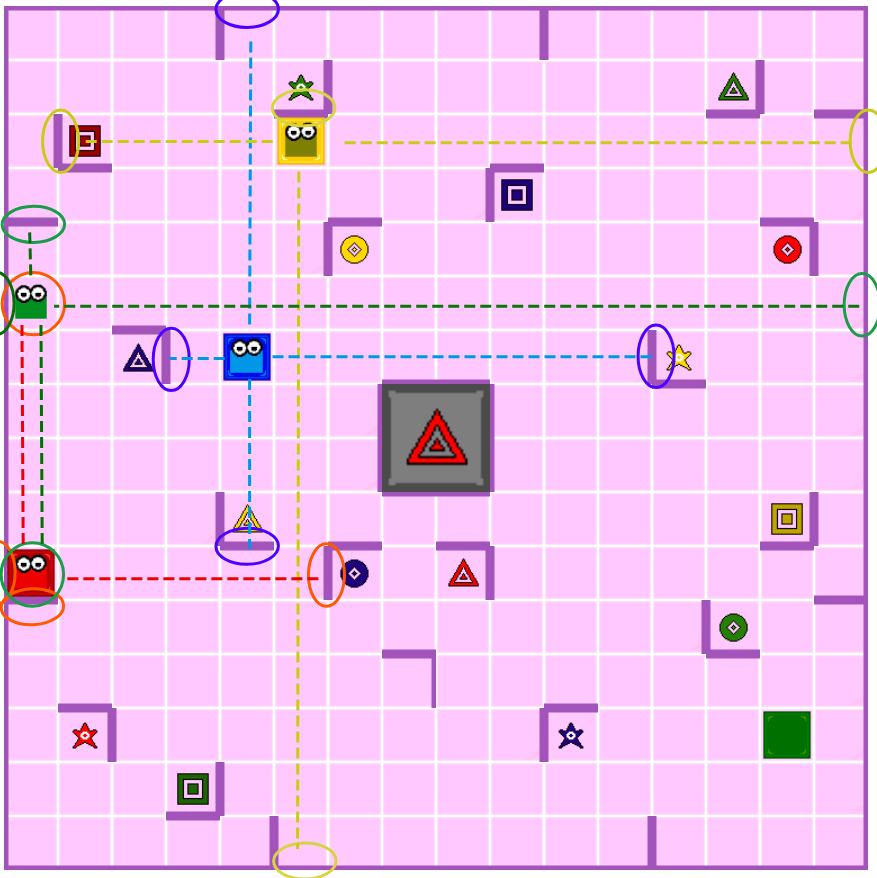
\includegraphics[scale=0.15]{Images/collision.png}
            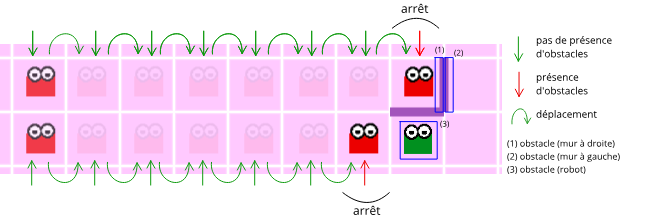
\includegraphics[scale = 0.4]{Images/deplacements.png}
        \end{frame}
        
%---------------------------------------------------------------        
\section{Interface Graphique}
    \begin{frame}{Représentation graphique}
        \begin{block}{L'interface est composée:}
            \begin{itemize}
                \item Des 4 robots avec leur couleur respectives.
                \item De la cible.
                \item De trois boutons \textbf{\textit{START,NEXT,RESET }}
                \item Du nombre de moves nécessaire pour atteindre la cible
            \end{itemize}
        \end{block}
    \end{frame}
%---------------------------------------------------------------     
    \begin{frame}{Représentation graphique}
        \begin{figure}
            \centering
            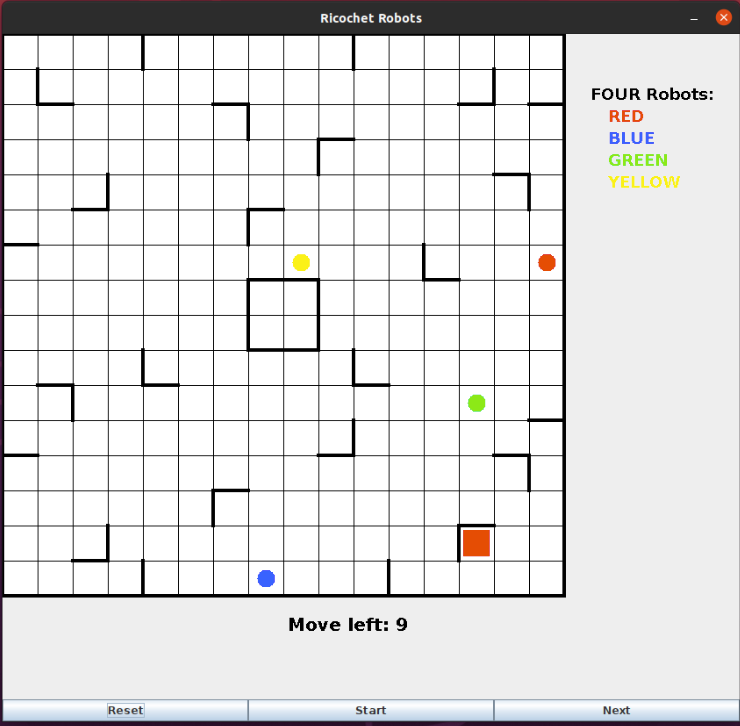
\includegraphics[scale=0.3]{Images/board.png}
        \end{figure}
    \end{frame}

%---------------------------------------------------------------
\section{Algorithme A*}
    \subsection{Présentation}
    \begin{frame}{Présentation}
       \begin{block}{AStar}
        \begin{itemize}
            \item A* aussi appelé \textbf{\textit{A - Star}} est un algorithme de parcours de graphe et de recherche de parcours.\\
            \item Il a été publié en 1968 par Peter Hart et Bertram Raphael.\cite{WikiAstar}.
            \item Peut être considéré comme une extension \textbf{\textit{Dijkstra}} \cite{WikiDijkstra}.
            \item A* parvient à obtenir de meilleurs résultats grâce à une heuristique guidant sa recherche.
        \end{itemize}   
       \end{block}
    \end{frame}
  
%---------------------------------------------------------------    
    \subsection{Optimisation}
        \begin{frame}{Pourquoi une heuristique?}
            \begin{itemize}
                \item Permet d'aller plus rapidement vers la solution.
                \item  Type d'heuristique le plus connu: heuristique du vol d'oiseau/distance euclidienne.
                
                \begin{itemize}
                    \item Calcule la distance du pion actuel par rapport à l'objectif
                    \item Priorise les états qui se rapprochent de l'objectif
                \end{itemize}
            \end{itemize}
            \begin{figure}
                \centering
                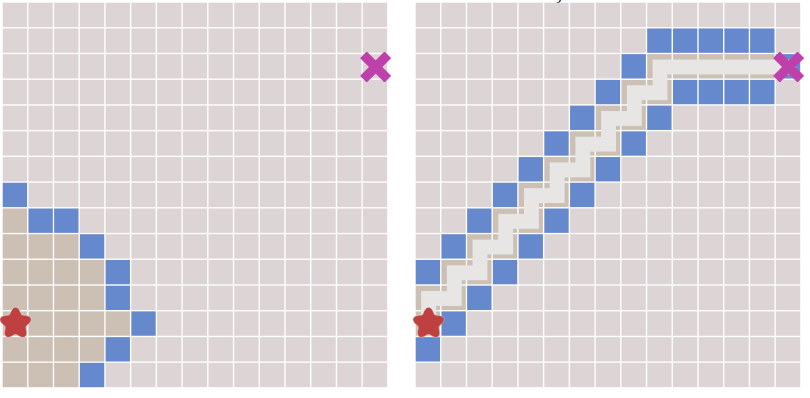
\includegraphics[scale=0.35]{Images/2.PNG}
                \caption{A* vs Dijkstra}
            \end{figure}
            Cependant, cette heuristique n'est pas optimale au Ricochet Robots.
        \end{frame}
        
%---------------------------------------------------------------        
    \subsection{Nouvelle Heuristique} 
    \begin{frame}{Mise en place}
        \centering
        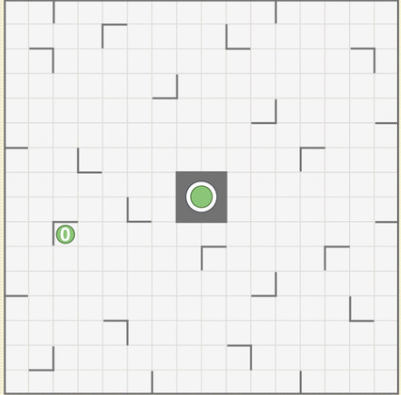
\includegraphics[scale=0.45]{Images/h1.png}
    \end{frame}
%---------------------------------------------------------------    
    \begin{frame}{1 Move de la cible}
        \centering
        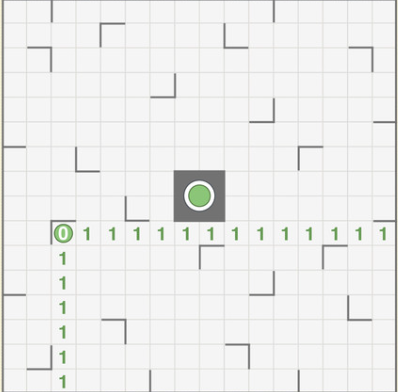
\includegraphics[scale=0.45]{Images/h11.png}
    \end{frame}
%---------------------------------------------------------------    
    \begin{frame}{2 Moves de la cible}
        \centering
        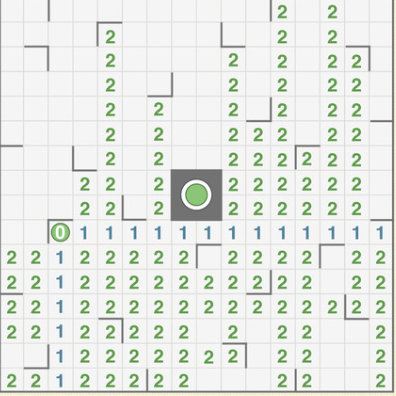
\includegraphics[scale=0.45]{Images/h2.png}
    \end{frame} 
%---------------------------------------------------------------    
    \begin{frame}{3 Moves de la cible}
        \centering
        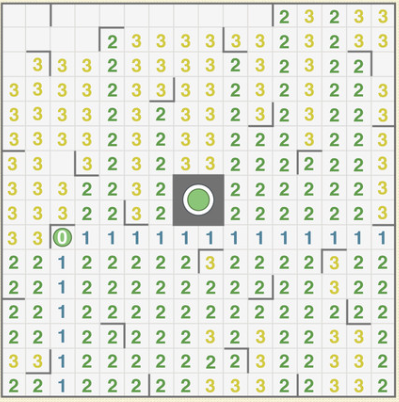
\includegraphics[scale=0.45]{Images/h3.png}
    \end{frame}
%---------------------------------------------------------------    
    \begin{frame}{4 Moves de la cible}
        \centering
        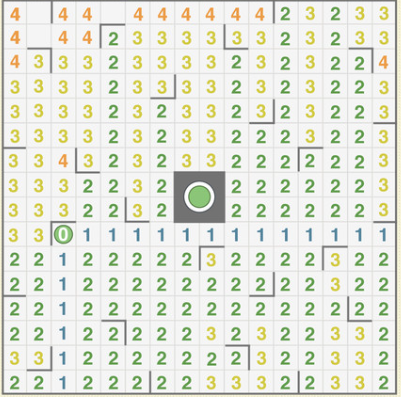
\includegraphics[scale=0.45]{Images/h4.png}
    \end{frame} 
%---------------------------------------------------------------    
    \begin{frame}{5 Moves de la cible}
        \begin{figure}
            \centering
            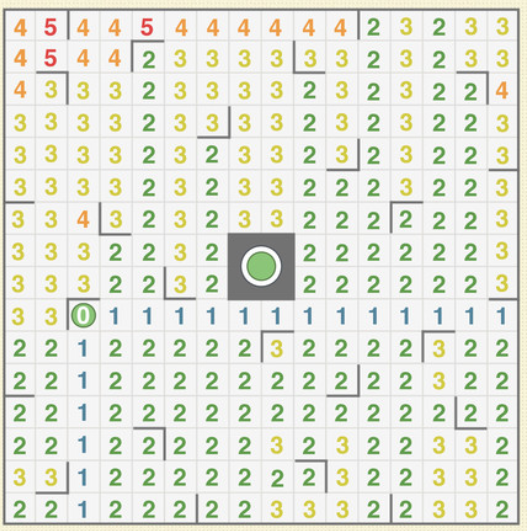
\includegraphics[scale=0.55]{Images/mapHeuristique.PNG}
            \caption{Tableau montrant en combien de mouvements à partir de chaque case on peut atteindre la cible \cite{heurist}}
            
        \end{figure}
    \end{frame}
%---------------------------------------------------------------    
    \subsection{Principe}
    \begin{frame}{FScore/GScore}
        \begin{itemize}
            \item Le prochain état a étudié est celui dont le coût jusque là (\textbf{\textit{GScore}}) + l'estimation
            du coût jusqu'à la cible (\textbf{\textit{Heuristique}}) est le \textbf{\textit{minimum}}.
        \end{itemize}
        \begin{figure}
            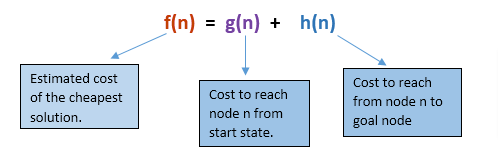
\includegraphics[scale=0.68]{Images/fn.png}
        \end{figure}
    \end{frame}
%---------------------------------------------------------------    
    \begin{frame}{Code}
        \scalebox{0.44}{    
        \begin{algorithm}[H]
            \caption{ALGORITHME ASTAR\_FINAL\_FORM}
            \SetKwInOut{Input}{Input}
            \SetKwInOut{Output}{Output}
            \Input{initialState, h}
            \Output{listOfStates}
            $openSet \gets \emptyset$ \\
            $priorityQueue \gets \emptyset$\\
            $gScore \gets \textbf{new}$ $map<State,Int>$ with \textbf{Default Value of +$\infty$ }\\
            $fScore \gets \textbf{new}$ $map<State,Int>$\\
            $startingState \gets initialState$\\
            $openSet.\textbf{add}(startingState)$\\
            $priorityQueue.\textbf{add}(startingState)$\\
            $gScore.\textbf{put}(startingState,0)$\\
            $fScore.\textbf{put}(startingState,h(startingState))$\\
            \While{$priorityQueue$ \textbf{is not empty}}{
                $currentState \gets priorityQueue.\textbf{poll()}$\\
                \If{$currentState.\textbf{isOver()}$}{
                    \Return{reconstructPath(cameFrom, currentState)}
                    }
                \tcc{On explore tous les états résultant d'un mouvement de robot}
                \ForEach{neighbor of currentState}{
                    $tentativeGscore \gets gScore[currentState] + 1$\\
                    \tcc{S'il est meilleur que tout ce que nous avions jusqu'à présent nous le gardons}
                    \If{$tentiveGscore < gScore[neighbor]$}{
                        $cameFrom[neighbor] \gets currentState$
                        $gScore[neighbor] \gets tentativeGscore$
                        $fScore[neighbor] \gets tentativeGscore + h(neighbor)$\\
                        \If{$neighbor$ $\textbf{not in openSet}$}{
                            $openSet.\textbf{add}(neighbor)$\\
                            $priorityQueue.\textbf{add}(neighbor)$\\
                        }
                    }
                }
            }
            \tcc{openSet est vide et la target jamais atteinte}
            $print(\textbf{"NO SOLUTION"})$\\
            \Return{$\emptyset$}
        \end{algorithm}

        \begin{algorithm}[H]
            \caption{ALGORITHME RECONSTRUCTPATH : RETOURNANT LE TRAJET}
            \SetKwInOut{Input}{Input}
            \SetKwInOut{Output}{Output}
            \Input{HashMap cameFrom<State,State>}
            \Input{currentState}
            \Output{ListOfStates}
            $listOfStates \gets \textbf{new}$ $List<State>()$\\
            $listOfStates.\textbf{add}(currentState)$\\
            \While{$currentState \in cameFrom.\textbf{Keys}$}{
                  $currentState \gets cameFrom.\textbf{get(currentState)}$\\
                  $listOfStates.\textbf{add}(currentState)$
            }
            \Return{listOfStates}
        
        \end{algorithm}
        }
    \end{frame}  
%---------------------------------------------------------------     

    \section{Démo}
        \begin{frame}{Démo}
            \centering
                Démonstration
        \end{frame}
%---------------------------------------------------------------
    
    \section{Conclusion}
        \begin{frame}{Conclusion}
            Ce projet était très intéressant. Nous ne connaissions pas le Ricochet Robots et c'était intéressant de se pencher sur les règles de ce jeu et de le recréer afin de pouvoir y jouer autrement que sous forme physique.
    
            \vspace{0.5cm}
            Améliorations possibles:
            \begin{itemize}
                \item Amélioration de  l'interface graphique, car l'interface finale est très basique.
		        \item Rajouter d'autres fonctionnalités comme pourvoir jouer par soi même.
		        \item Faire des tests comparant différents type d'algorithmes.
            \end{itemize}
        \end{frame}

%---------------------------------------------------------------
    \begin{frame}{Bibliographie}
        Références:
        \bibliographystyle{unsrt}
        \bibliography{bibliography}       
    \end{frame}    
\end{document}